\chapter{Đánh giá các thông số hiệu năng của mô hình nhận diện}
Mô hình được huấn luyện trong ba ngày với $12000$ iteration. Trong quá trình huấn luyện, việc tính toán các thông số hiệu năng của mô hình được thực hiện với mỗi $1000$ iteration trên tập dữ liệu validation. 
Nhắc lại về cách tính các thông số hiệu năng:
\begin{itemize}
	\item Precision là thông số thể hiện độ chính xác của các dự đoán. $True Positive$ (viết tắt: TP) là những bounding box được dán nhãn đúng và thực sự đúng. $False Positive$ (viết tắt: FP) là những bounding box được dán nhãn đúng và không thực sự đúng. Precision được tính bằng công thức
	\begin{equation}
		precision = \frac{TP}{TP+FP}
	\end{equation}
	\item Recall là thông số thể hiện độ nhạy của mô hình với các đối tượng cần nhận dạng. $True Positive$ (viết tắt: TP) là những bounding box được dán nhãn đúng và thực sự đúng. $False Negative$ (viết tắt: FN) là những bounding box được dán nhãn không đúng hoặc không được dán nhãn và thực sự đúng. Recall được tính bằng công thức
	\begin{equation}
		precision = \frac{TP}{TP+FN}
	\end{equation}
	\item Average precision là thông số được tính cho một class. Với mỗi class, trong quá trình đánh giá trên tập dữ liệu validation, các giá trị precision và recall sẽ được lưu lại. Sau đó ta sẽ vẽ đồ thị của precision theo recall, average precision của một class sẽ là phần diện tích dưới đồ thị này. Gọi $p(r):[0,1]\rightarrow[0,1]$ là hàm số biểu diễn quan hệ của precision và recall. Average precision của một class sẽ được tính theo công thức
	\begin{equation}
		\text{average precision} = \int_{0}^{1} p(r) dr
	\end{equation}
	\item Mean average precision là trung bình của các average precision của các class
	\begin{equation}
		\text{mean average precision} = \frac{\sum_{i=0}^{N} ap_i}{N}
	\end{equation}
	Với $N \in \mathbb{N}^*$ là số class của mô hình.
\end{itemize}

Tập dữ liệu validation gồm $900$ hình được chia một cách ngẫu nhiên từ tập dữ liệu gốc và không được dùng để huấn luyện, số lượng các object trong tập dữ liệu này được thể hiện trong hình \ref{fig:validation_set}
\begin{figure}[ht!]
	\centerline{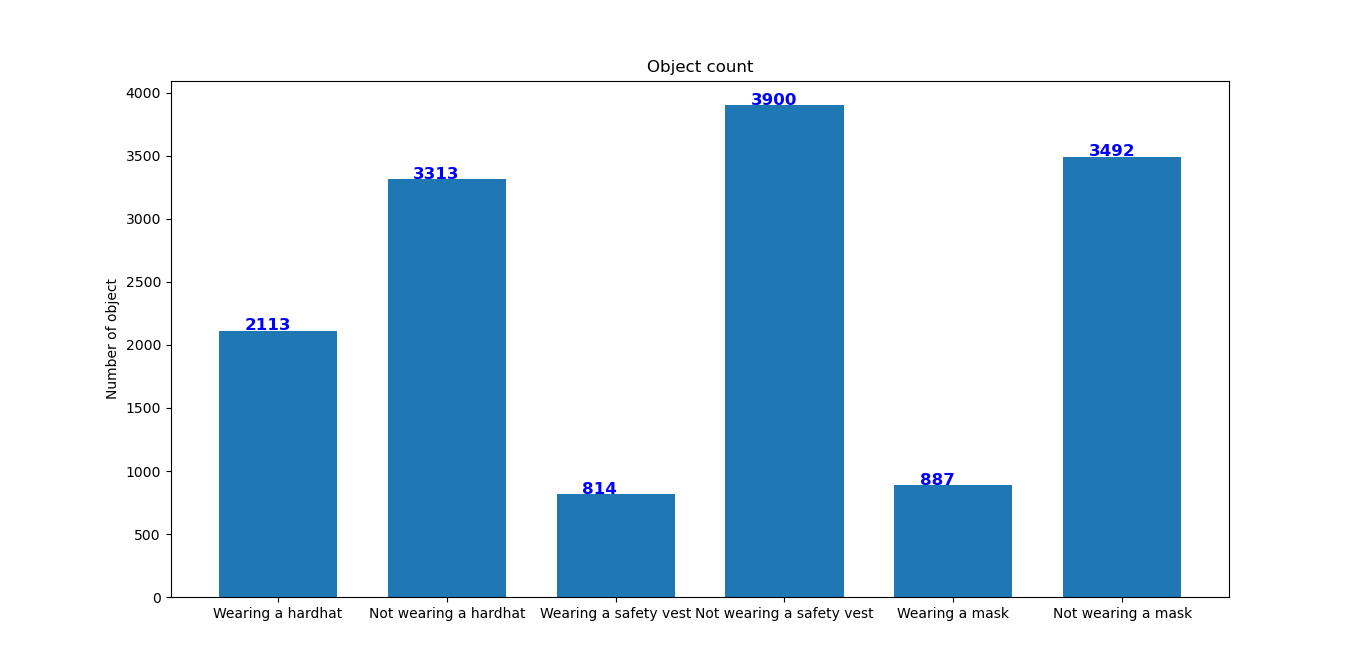
\includegraphics[scale=0.5]{images/validation_set.png}}
  	\caption{Số lượng các object trong tập dữ liệu validation. Wearing a hardhat - $2113$, Not wearing a hardhat - $3313$, Wearing a safety vest - $814$, Not wearing a safety vest - $3900$, Wearing a mask - $887$, Not wearing a mask - $3492$.}
  	\label{fig:validation_set}
\end{figure}

Các thông số được tính toán gồm: precision, recall và mean average precision \ref{fig:precision_recall_map}.
\begin{figure}[ht!]
	\centerline{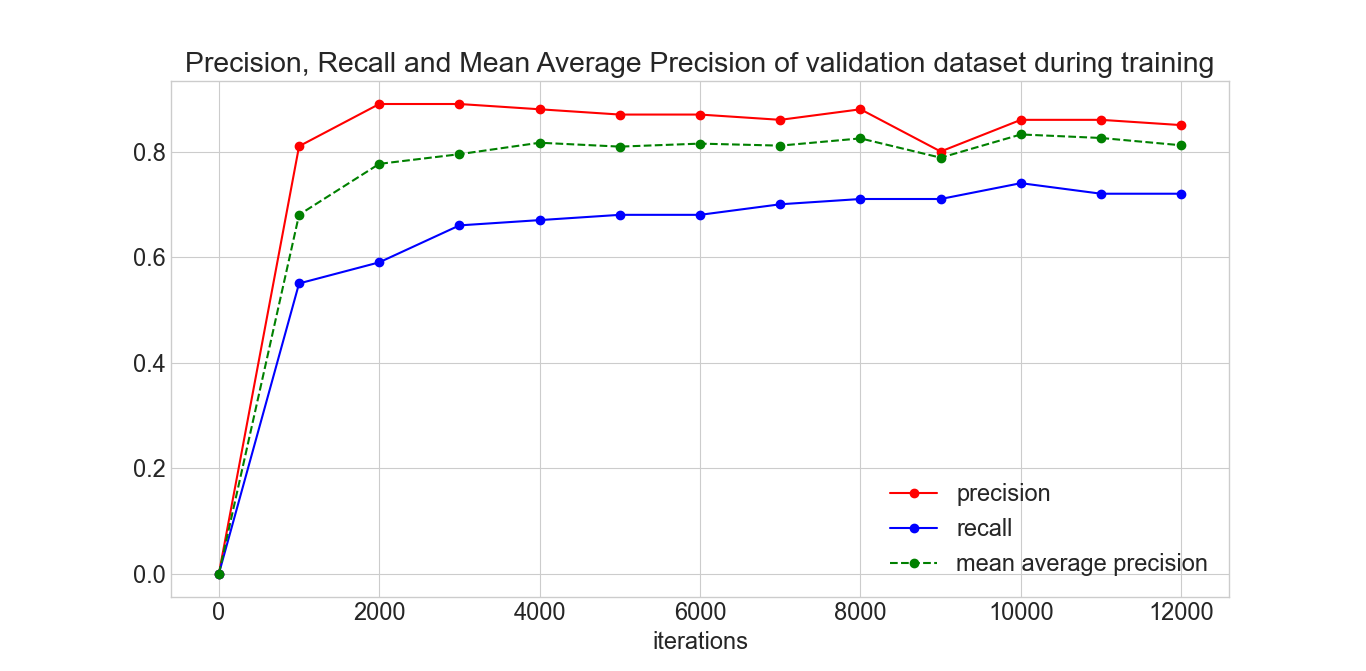
\includegraphics[scale=0.6]{images/precision_recall_map.png}}
  	\caption{Precision - màu đỏ, Recall - màu xanh dương, Mean Average Precision - màu xanh lá. Các thông số được tính toán mỗi 1000 iteration trên tập dữ liệu validation.}
  	\label{fig:precision_recall_map}
\end{figure}

Một số kết quả của mô hình khi dự đoán trên hình:
\begin{figure}[ht!]
	\centerline{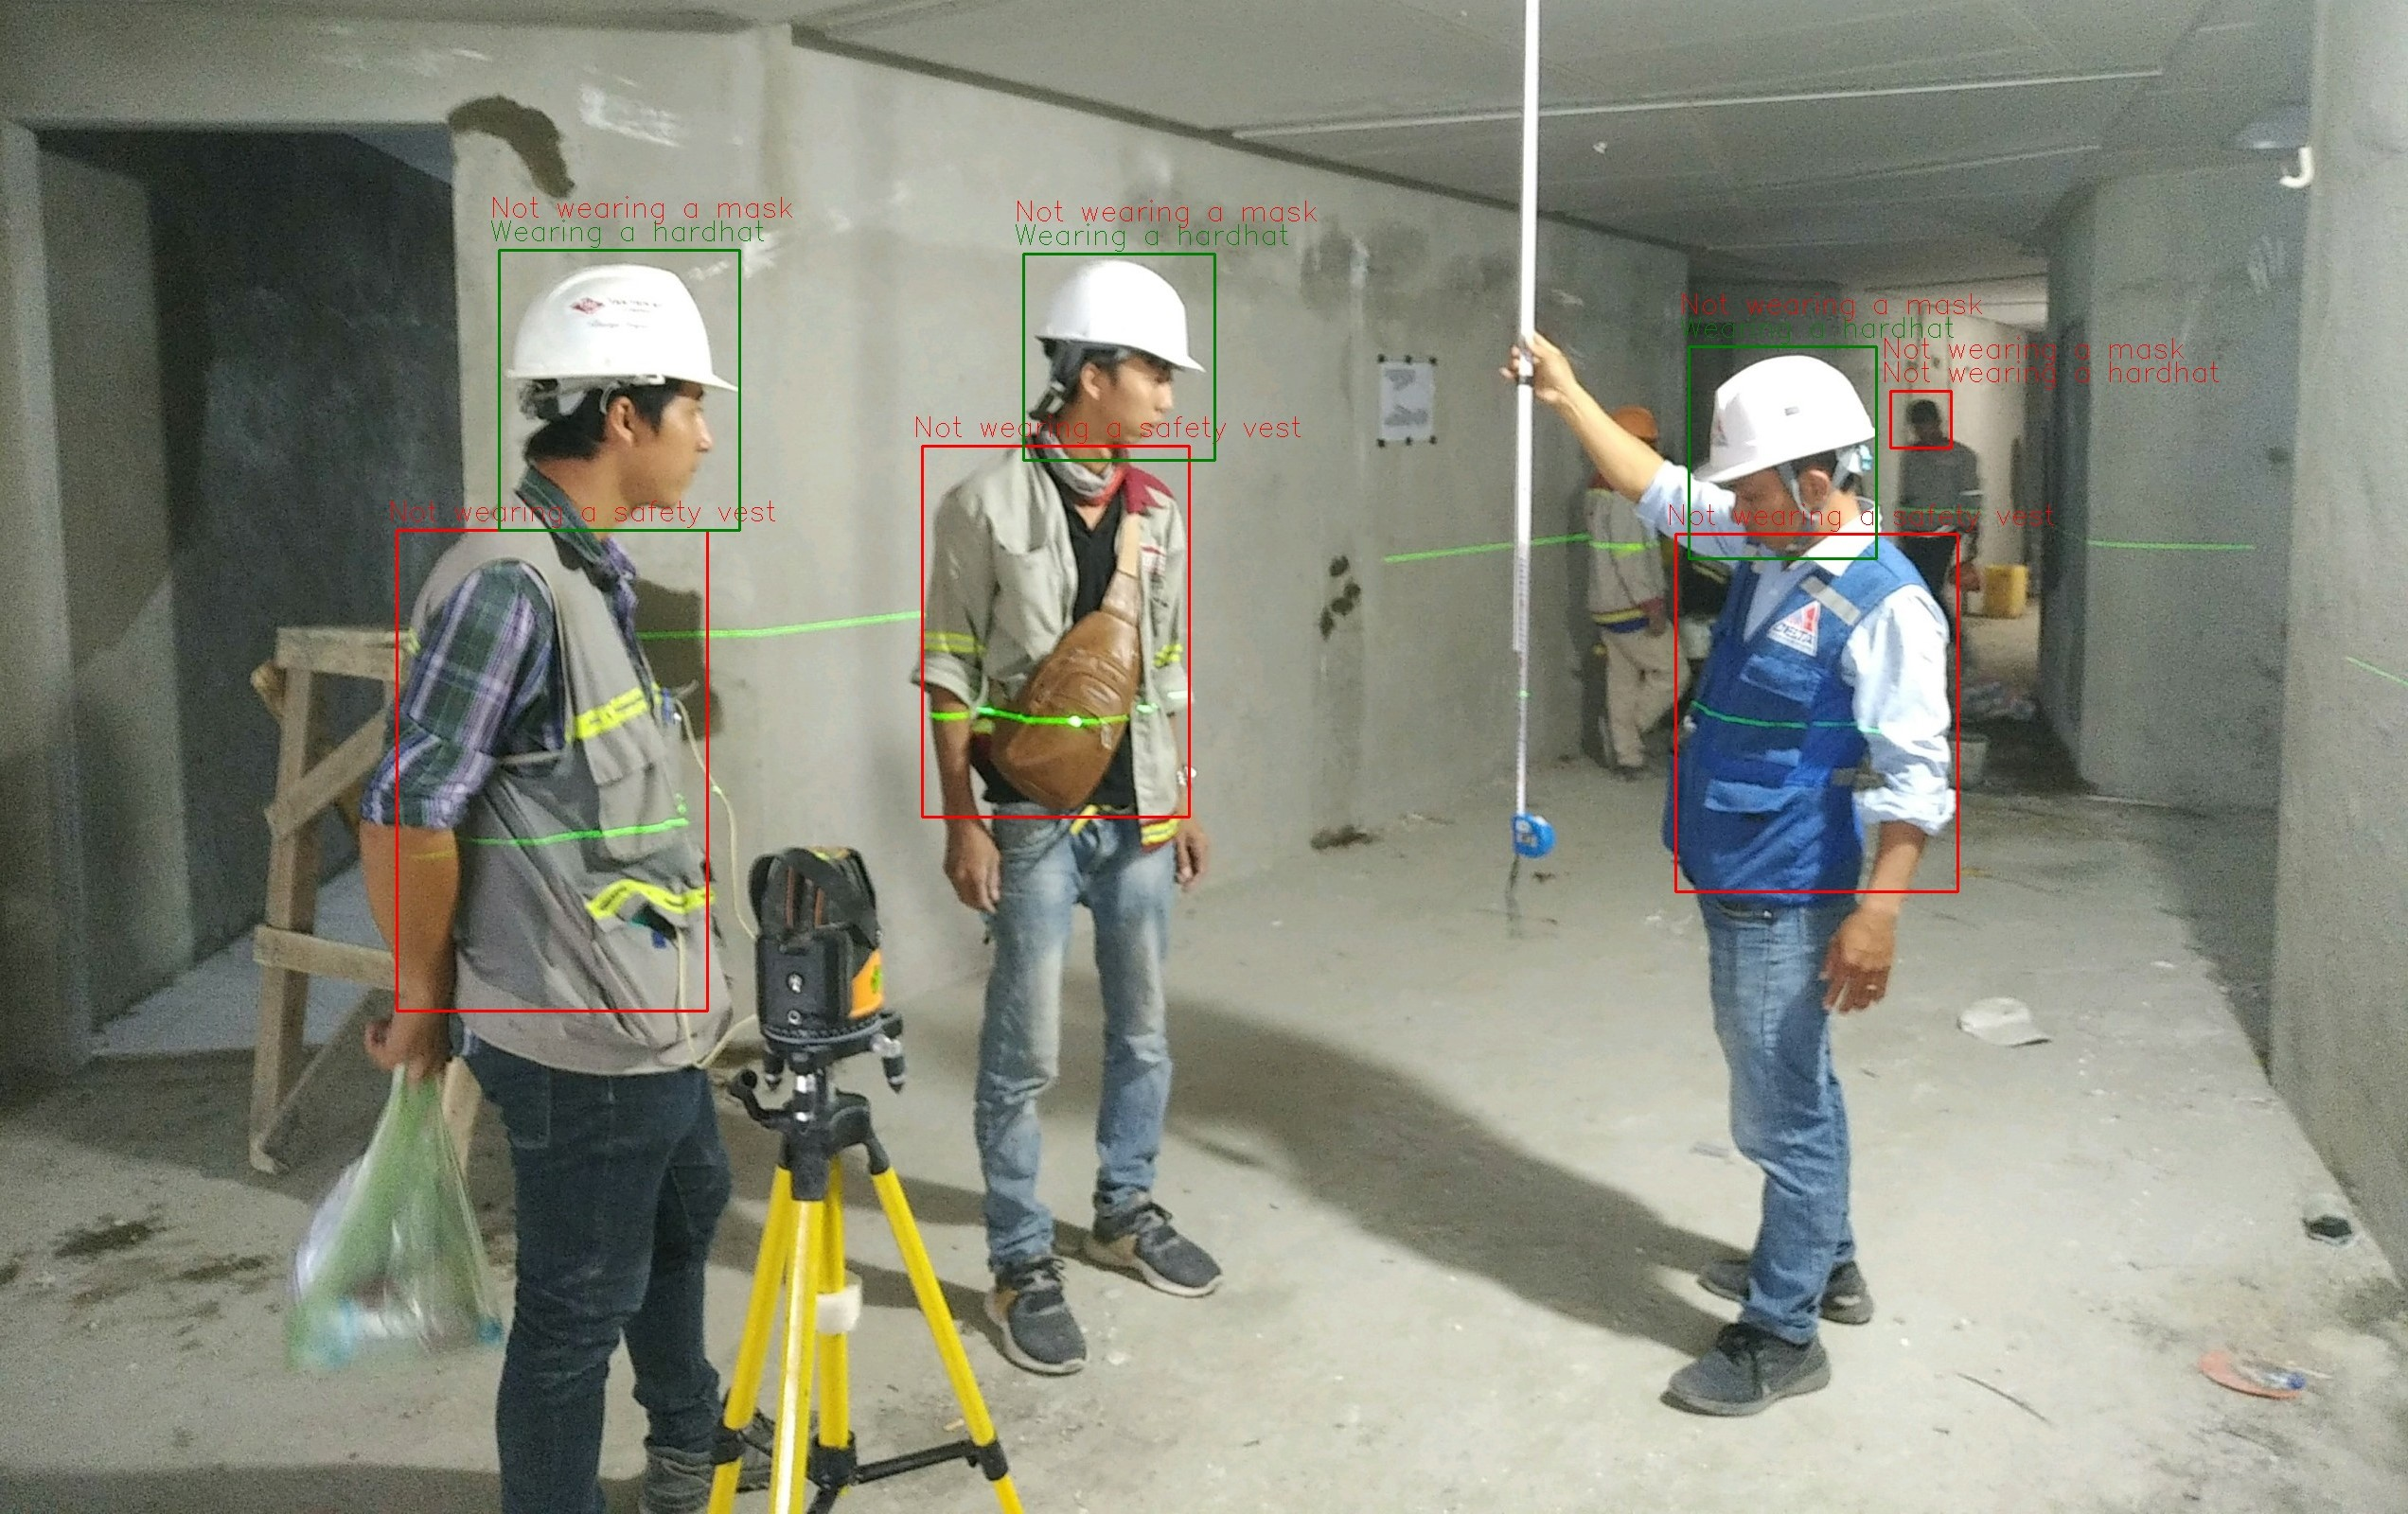
\includegraphics[scale=0.2]{images/result_2.jpg}}
	\centerline{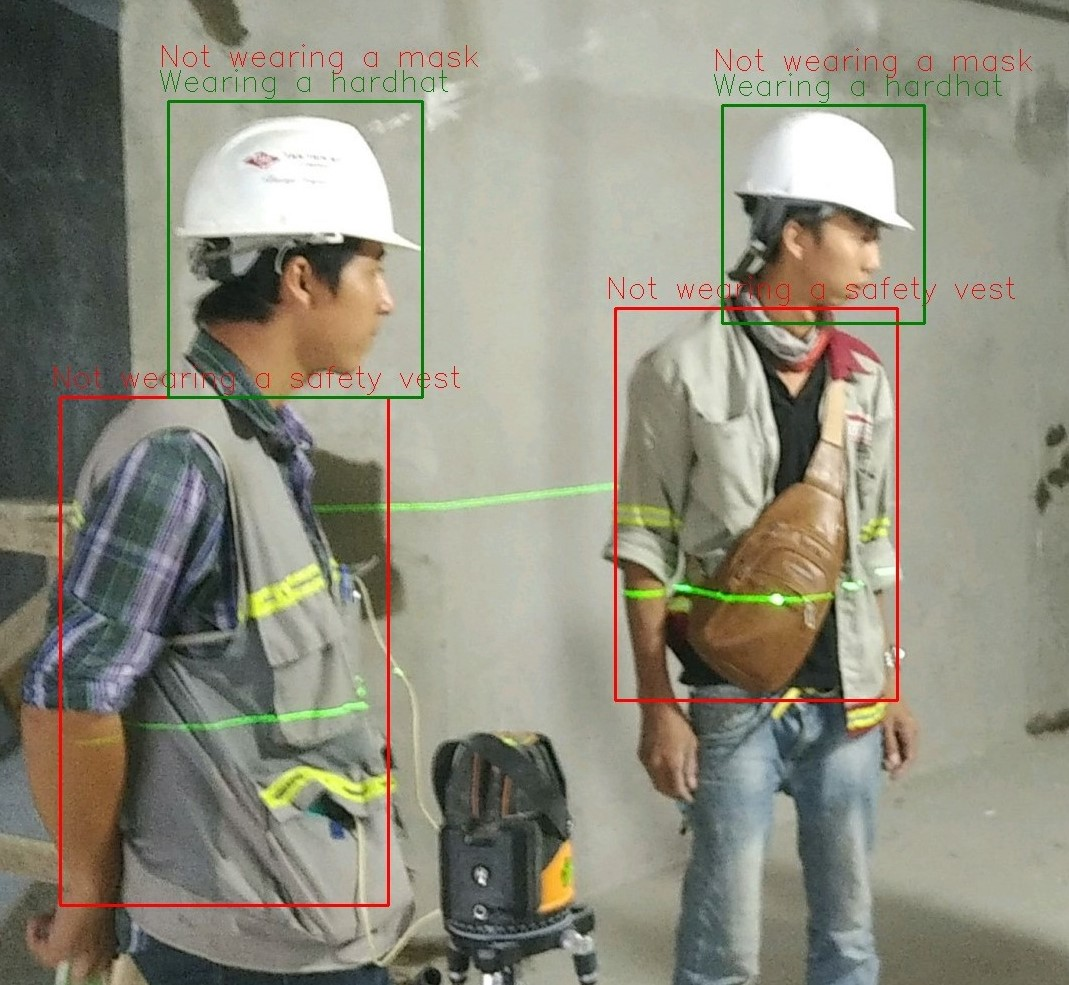
\includegraphics[scale=0.37]{images/result_2a.jpg}}
  	\caption{Kết quả dự đoán tốt - hình trên. Phóng to một phần của kết quả dự đoán - hình dưới.}
  	\label{fig:precision_recall_map}
\end{figure}
\begin{figure}[ht!]
	\centerline{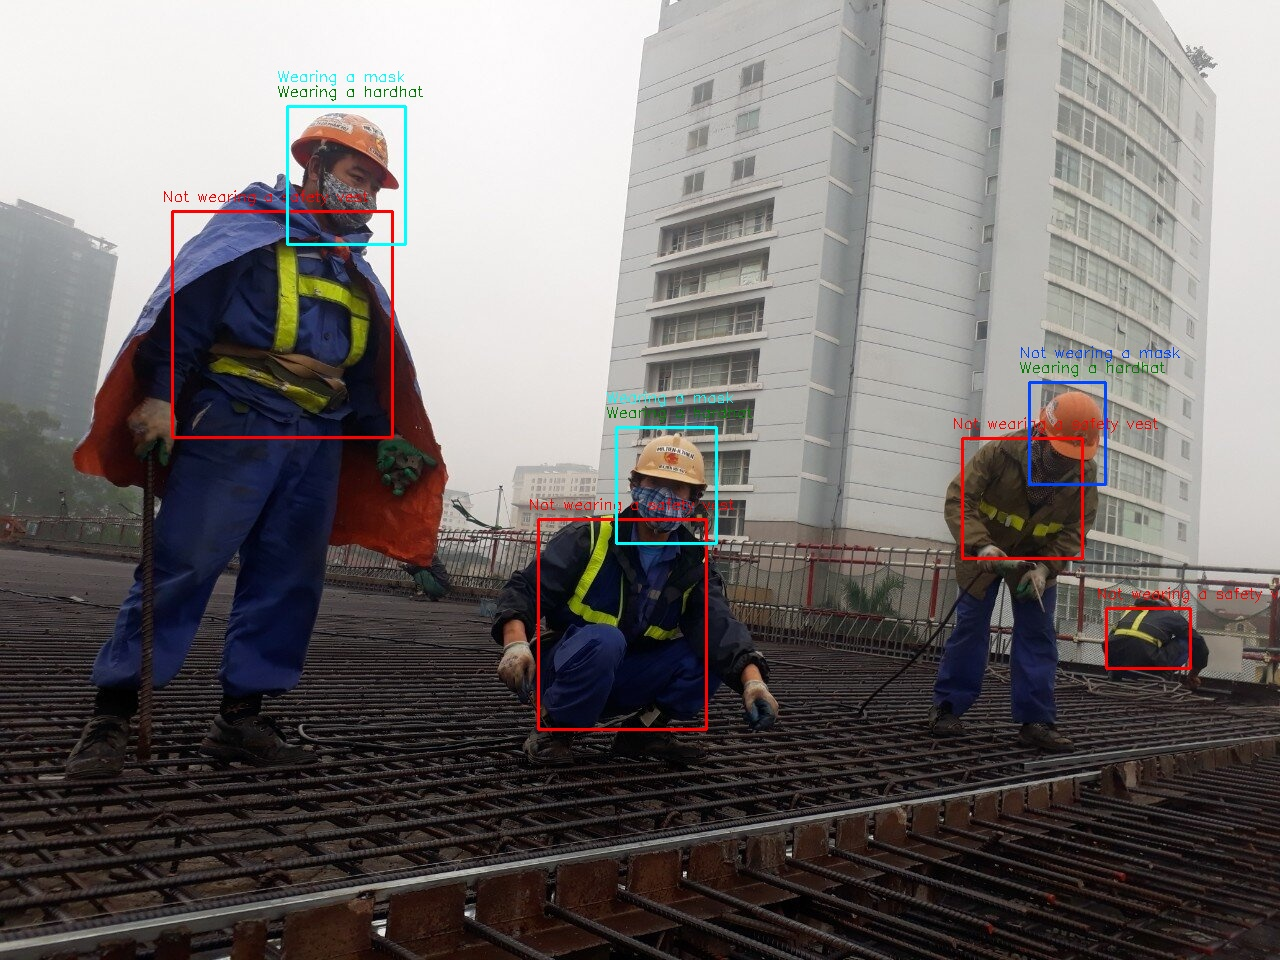
\includegraphics[scale=0.25]{images/result_1.jpg}}
	\centerline{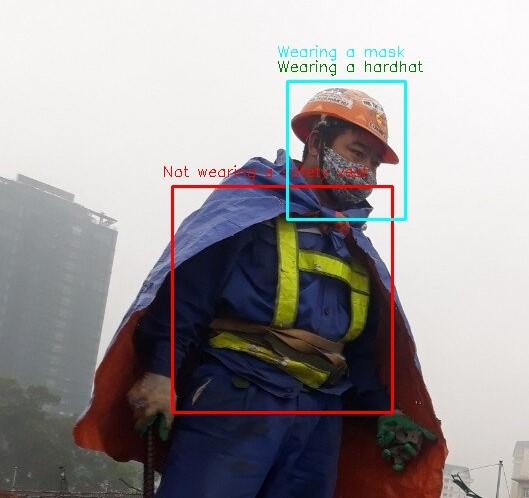
\includegraphics[scale=0.6]{images/result_1a.jpg}}
  	\caption{Kết quả dự đoán tốt - hình trên. Phóng to một phần của kết quả dự đoán - hình dưới.}
  	\label{fig:precision_recall_map}
\end{figure}
\begin{figure}[ht!]
	\centerline{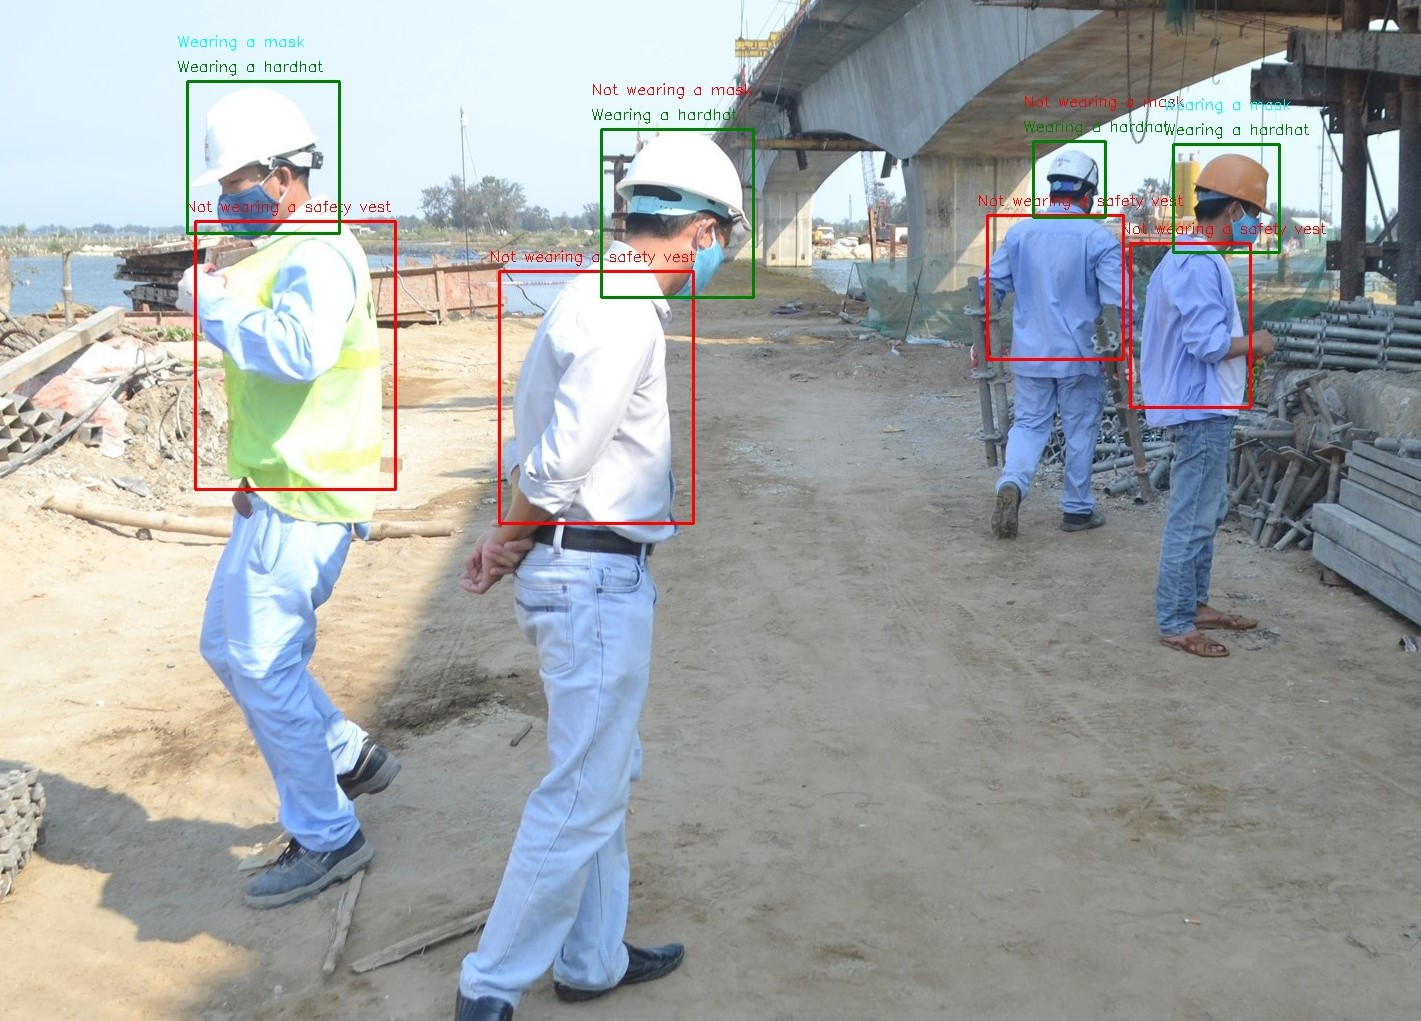
\includegraphics[scale=0.3]{images/result_3.jpg}}
	\centerline{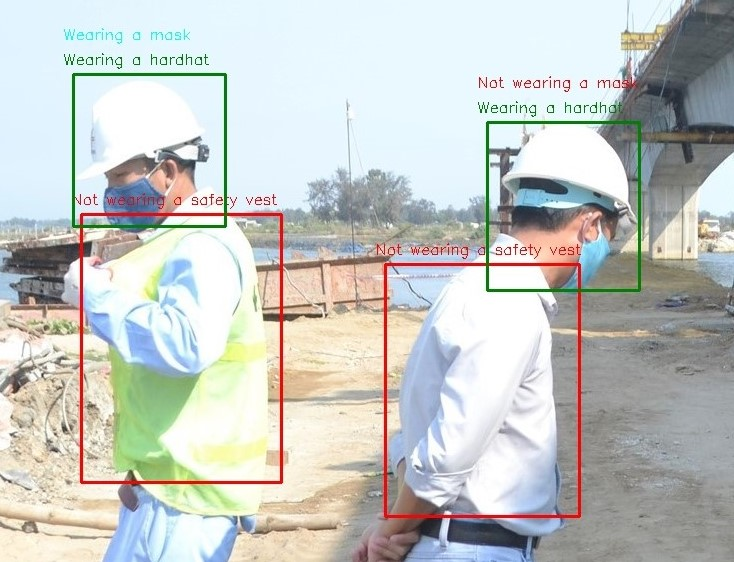
\includegraphics[scale=0.6]{images/result_3a.jpg}}
  	\caption{Kết quả dự đoán không tốt - hình trên. Phóng to một phần của kết quả dự đoán - hình dưới.}
  	\label{fig:precision_recall_map}
\end{figure}
\begin{figure}[ht!]
	\centerline{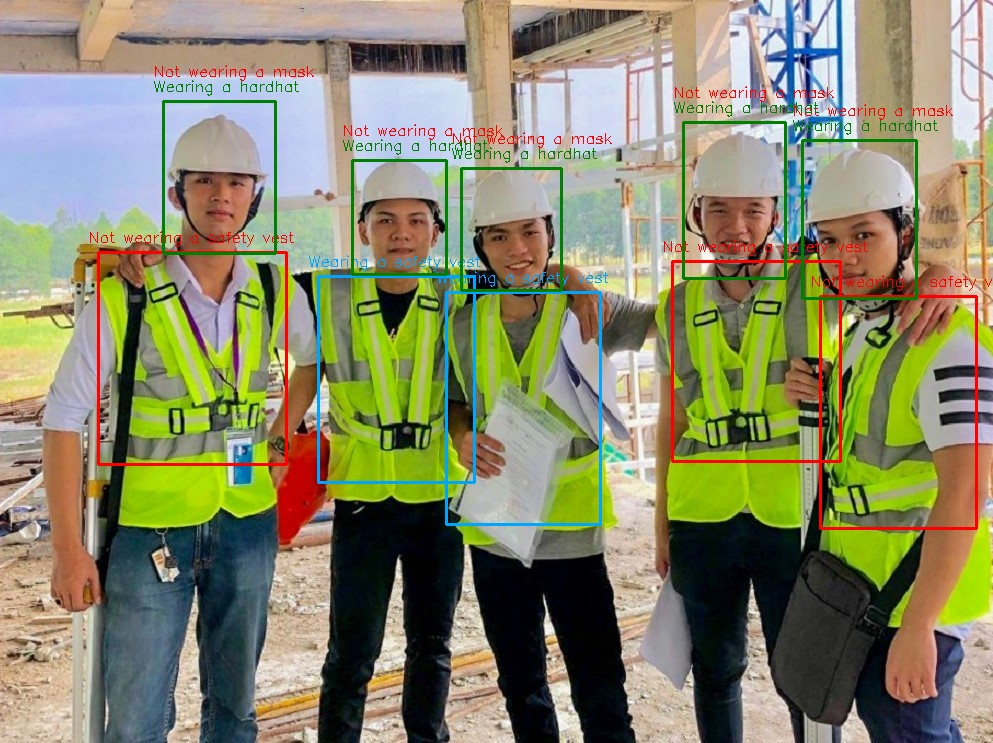
\includegraphics[scale=0.3]{images/result_4.jpg}}
	\centerline{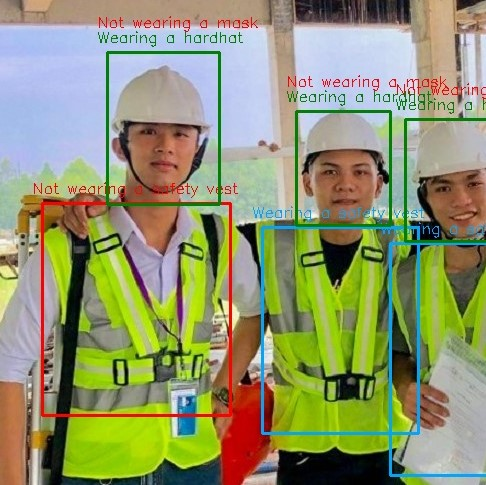
\includegraphics[scale=0.6]{images/result_4a.jpg}}
  	\caption{Kết quả dự đoán không tốt - hình trên. Phóng to một phần của kết quả dự đoán - hình dưới.}
  	\label{fig:precision_recall_map}
\end{figure}

\textbf{Nhận xét}: Mô hình có thể phát hiện rất tốt các vị trí cần nhận diện gồm phần đầu và cơ thể. Đồng thời có khả năng phân loại tương đối tốt với các vật thể được phát hiện. Tuy nhiên đối với một số class mang đặc tính \textit{wearing} thì đôi khi vẫn bị nhầm lẫn với các class \textit{not wearing}. Điều này có thể xuất phát từ vị trí góc nghiêng của vật thể được phát hiện không cho phép mô hình đưa ra dự đoán chính xác.